\subsection{The domain: \naze, Portugal}
\label{sec:naz}

\begin{figure}[!b]
  \vspace{-0.5cm} 
  \centering 
  \subfigure[Map of Portugal and the study area highlighted with the red
  rectangle.]{\label{fig:po-map}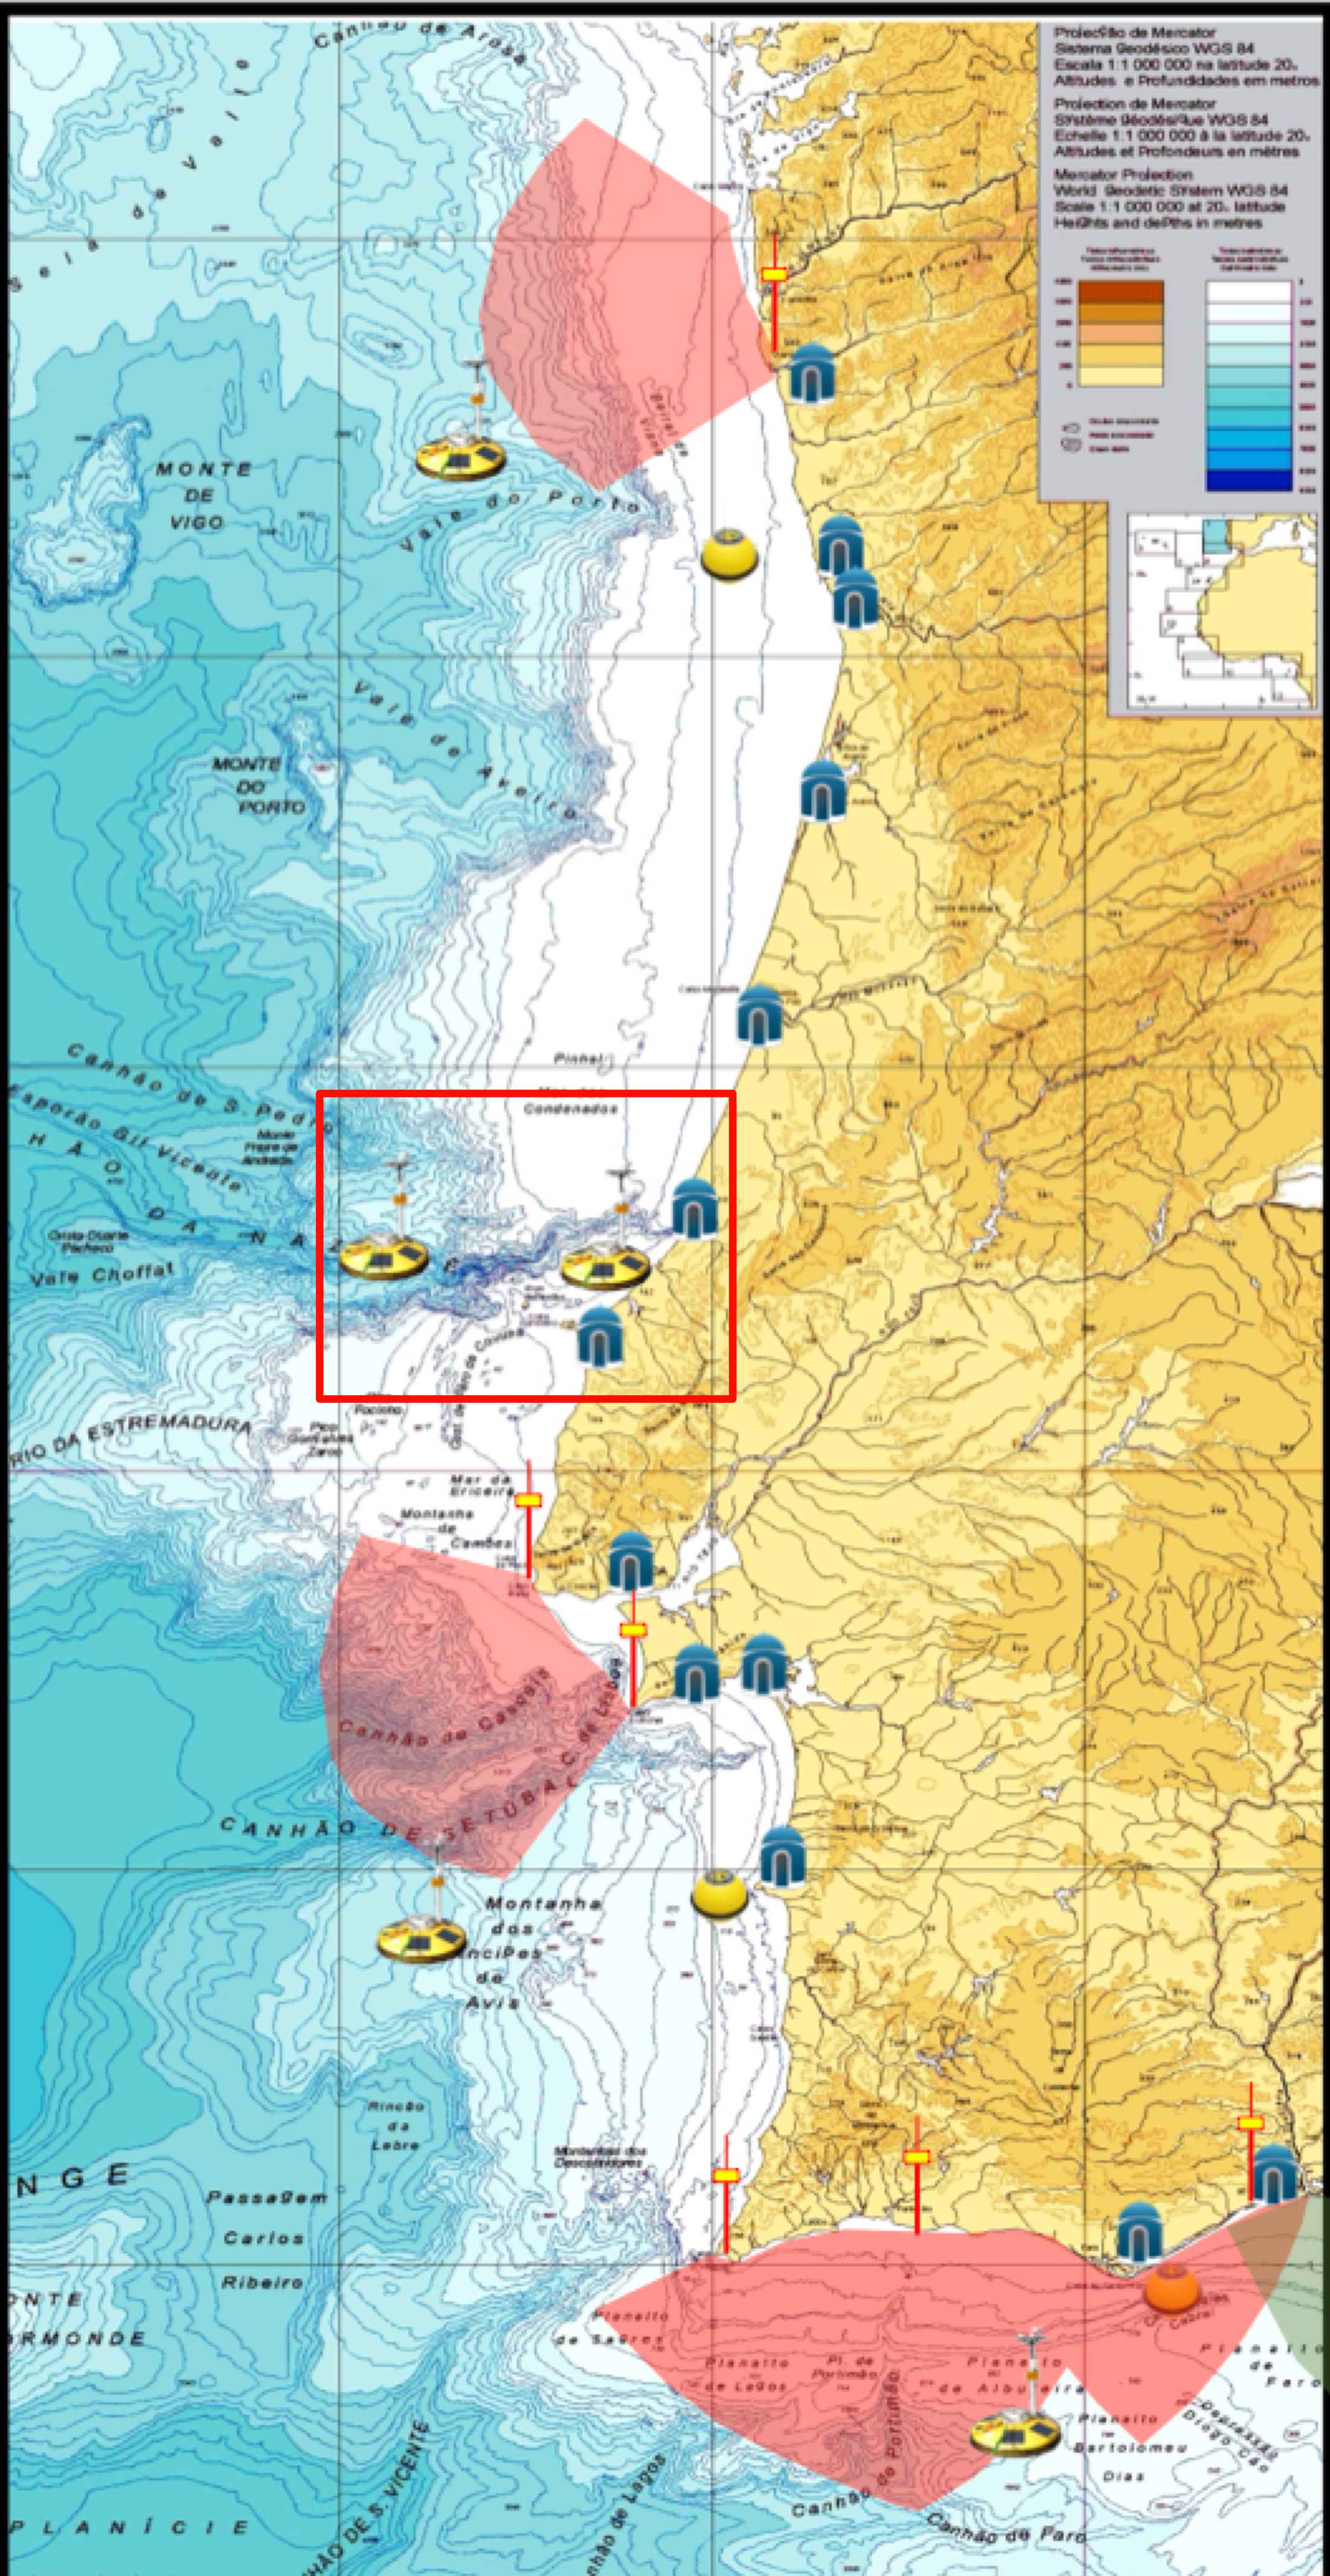
\includegraphics[scale=0.5]{fig/po-map.jpeg}}
  \hspace{+0.3cm} 
  \subfigure[Zoomed in bathymetry showing the \naz canyon-Berlengas
  area (isobaths with depth in meters) and its environment including
  the placement of the two buoys.]{\label{fig:domain}\includegraphics[scale=0.55]{fig/domain.jpg}}
  \caption{\subref{fig:po-map} \& \subref{fig:domain} show detailed
    views of the proposed study area for \proj off the coast of
    mainland Portugal. The \naz Canyon is a significant feature of
    this area and a driver for the bio-geophysics of the domain. The
    shaded blue area is the expected glider operations region which
    will inform the model about boundary conditions and off-shore
    waters being entrained into the canyon.}
  \label{fig:studyarea-1}
\end{figure}

\proj will focus on the area of influence of \naz Canyon located in
the central part of the western Portuguese coast and broadly extending
from 39.2$^{\circ}$N (south of Peniche) to 39.9$^{\circ}$N north of
\naz (Fig. \ref{fig:po-map}). This is a coastal ocean area well
exposed to the influence of the North Atlantic and marked by
important topographic features such as:

\begin{itemize}[noitemsep,topsep=0pt,parsep=0pt,partopsep=0pt]

\item important changes of the continental margin associated with the
  transition from the large Estremadura Plateau to the south, to the
  relatively narrow shelf north of \naz

\item the presence of a long and narrow submarine \naz canyon that
  extends for more than 200 km from the head, just a few hundreds of
  meters from the beach of \naze, incising the shelf into the abyssal
  area

\item the presence of island environments -– the Berlengas archipelago
  located a few tens of kilometers offshore the coast which is a
  \texttt{Natura2000} site recognized as a unique repository of
  species and habitat diversity on the western boundary of Europe. It
  was recently classified by UNESCO as a Biosphere Reserve. The
  biogeographic, geologic and oceanographic settings of this region,
  accentuated by the presence of the \naz canyon, are critical for the
  high levels of biological productivity and biodiversity, that induce
  dynamic ecological processes and support many ecosystem services

\end{itemize}


\vspace{+0.5cm}
The \naz Canyon area of influence is not directly impacted by major
riverine outflows. The main rivers influencing the western Portuguese
continental margin are the Douro (located about 170 km to the north of
\naze) and the Tagus (located at about 100 km to the south) with
smaller contributions from the Mondego (50 km to the north). During
the winter and early spring the combined influence of the Douro and
other smaller rivers such as the Mondego reach the \naz Canyon area
during periods of northerly winds and upwelling conditions, appearing
as a low salinity water plume occupying the first 30 m of the water
column and extending over the complete shelf as the result of offshore
transport associated with the prevailing upwelling conditions. The
influence of the Tagus River on the area is less clear, largely due to
the combination of the large Estremadura Plateau with the shallow
ridge between Cape Carvoeiro and Berlengas areas and associated
circulation characteristics. More expressive for the conditions in the
area is the contribution of the small riverine sources that indent the
\naze-Peniche coast during periods of important precipitation. These
include the contributions of the small Alcoa and Tornadas rivers, of a
large number of very small fresh water courses (ribeiras) or from the
Obidos Lagoon. Previous observations have showed \cite{martins10} that
these contributions combine fresh waters with high turbidity and high
nutrient content that can extend its influence over the complete
shelf.

The evolution of wind forcing and wave conditions affecting this area
is largely determined by the seasonal migration of the Azores High
Pressure System. From May to September the Azores High is typically
located at its northernmost position, offshore the Iberian
Peninsula. During this period, the western Portuguese margin is
located on the eastern branch of the High, under the influence of
persistent (upwelling favorable) northerly winds that during the
summer months, are reinforced by the establishment of a thermal low
over central Iberia. The area is also protected from the influence of
synoptic low pressure systems, showing typically low energy swells
(although affected by locally generated sea breeze
circulation). During the winter months the conditions prevailing along
the western Portuguese margin are largely associated with the phase of
the winter North Atlantic Oscillation (NAO). During the negative phase
of the winter NAO the Azores High is typically located southwest of
the Iberian Peninsula and the western Portuguese coast is under the
influence of westerly and southwesterly wind forcing that frequently
promote downwelling conditions. During those periods the area is also
exposed to the direct influence of synoptic low pressure systems and
associated highly energetic waves. During the positive phases of the
winter NAO, the Azores High remains at northward latitudes leading to
frequent periods of northerly winds and upwelling conditions along the
western Portuguese margin. During these periods the area is largely
protected from the direct influence of low pressure synoptic systems
and shows a less energetic wave regime in general, although impacted
by large swells that are generated far in the North Atlantic.

The atmospheric forcing conditions described above establish some
complex dynamics in the \naz canyon area of influence, marked by the
interactions of the shelf and slope circulation with the canyon
topography and island environments and by the manifestation of
important meso-scale features such as the upwelling filament of Cape
Carvoeiro. In addition, the rich topography of the area also promotes
complex tidal dynamics. Barotropic tidal currents along the western
Portuguese margin are in general dominated by the semidiurnal lunar
constituent (M2), within a period of 12 hours and 25 minutes.  In the
shelf north of \naz canyon the barotropic tidal current magnitudes are
dominated by the M2 constituent and show magnitudes of 5-10 cm/s. To
the south of Peniche, the large and shallow Estremadura Plateau
constitutes an area of intensification of the barotropic tidal
currents, both for the dominant constituent (M2) that shows magnitudes
of order 10 cm/s, as well as for the diurnal constituents such as the
lunar diurnal constituent (K1) that shows magnitudes comparable with
M2 \cite{marta06,quaresma13}. A particular area of interest, is the
shallow ridge located between Cape Carvoeiro and Berlengas Islands
where total currents can on some occasion, reach 50-60 cm/s.


The interaction of the barotropic tide with the shelf edge topography
in the presence of stratification opens the potential for generation
of internal tidal motions that propagate offshore to the deep ocean
domain and, if the stratification conditions of the continental shelf
allow, also onshore. The effect of these internal motions generated at
the shelf edge however remains largely confined to the outer and
mid-shelf, the waves being dissipated before reaching the inner shelf
environment. By cutting the complete continental shelf, the \naz
canyon opens the possibility for internal tidal motions to be
generated at positions along the canyon rim located very close to the
shore, impacting the mid and inner shelf environments if
stratification conditions allow the onshore propagation of these
waves. An example of those impacts was presented by \cite{quaresma07}
based on observations of solitons generated at the canyon rim and
propagating towards the inner continental shelf impacting the bottom
sedimentary cover and promoting vertical mixing.
